\part{Wave-Based Semantic Representation}

\chapter{Complex-Valued Semantic States}\label{ch:complex}

The wave-based proposal of Listopad models each semantic pattern as a discrete complex-valued waveform
\begin{equation}\label{eq:wave}
\psi(x)=A(x)\,e^{\iu\phi(x)},\qquad A(x)\ge 0,\quad \phi(x)\in[-\pi,\pi),
\end{equation}
where $x$ indexes the coordinates of the pattern, $A$ is an amplitude that the source interprets as semantic intensity or salience, and $\phi$ is a phase that the source interprets as contextual or operator-level modulation \cite{listopad2025}. The generalization used here replaces the coordinate index by an arbitrary index set and the pattern by an element of a complex Hilbert space $\Hil$, with inner product $\ip{\psi}{q}=\sum_x\overline{\psi(x)}\,q(x)$ in the finite-dimensional case, linear in the second argument. Individual traces are vectors $m_i\in\Hil$, and the representation above is recovered by writing each coordinate in polar form.

The basic quantities are standard but must be fixed because the later arguments depend on exactly which of them a given score uses. The energy of a pattern is $E(\psi)=\norm{\psi}^2=\sum_x|\psi(x)|^2=\sum_xA(x)^2$, which is independent of phase. The inner product splits into a real and an imaginary part, $\ip{\psi}{q}=\Re\ip{\psi}{q}+\iu\,\Im\ip{\psi}{q}$, and the real part carries the sign-sensitive agreement between the two patterns coordinate by coordinate: $\Re\ip{\psi}{q}=\sum_xA_\psi(x)A_q(x)\cos(\phi_q(x)-\phi_\psi(x))$. Interference between two patterns, the squared norm of their sum, satisfies $\norm{\psi+q}^2=\norm{\psi}^2+\norm{q}^2+2\Re\ip{\psi}{q}$, which is the algebraic content of the statement that waves in phase reinforce and waves in antiphase cancel. Coherence is used here in a precise sense: the modulus of the normalized inner product, $\kappa(\psi,q)=|\ip{\psi}{q}|/(\norm{\psi}\norm{q})\in[0,1]$, measures the degree of alignment up to a single global phase, while the normalized real part $c(\psi,q)=\Re\ip{\psi}{q}/(\norm{\psi}\norm{q})\in[-1,1]$ measures alignment including the phase offset. A pattern and a copy of it multiplied by $e^{\iu\alpha}$ have coherence $1$ and phase-aware agreement $\cos\alpha$.

The distinction between phase as an encoding convention and phase as a dynamically meaningful relational variable can now be stated exactly. Multiplication of every pattern in a system by the same unit complex number $e^{\iu\alpha}$ is a gauge transformation: it changes every vector and no observable that depends only on norms and on $|\ip{\psi}{q}|$, and it changes no quantity that depends only on $\Re\ip{\psi}{q}$ computed between two patterns transformed together. Phase is therefore a convention to the extent that only global phase is arbitrary. Phase is a relational variable to the extent that relative phases between components, or between a query and a stored pattern, change the outcome of a computation. The distinction matters because a representation in which phase carries information is only as good as the discipline that keeps phases comparable across encodings: if the encoder of a pattern and the encoder of a query assign phases by different conventions, the relative phase between them is an artifact and the score it modulates is noise.

\begin{proposition}[Gauge invariance]\label{prop:gauge}
Let $U_\alpha\psi=e^{\iu\alpha}\psi$. Then $\ip{U_\alpha\psi}{U_\alpha q}=\ip{\psi}{q}$ for every $\alpha$, while $\ip{U_\alpha\psi}{q}=e^{-\iu\alpha}\ip{\psi}{q}$. In particular $|\ip{\psi}{q}|$ is invariant under independent phase changes of the two arguments, and $\Re\ip{\psi}{q}$ is invariant only under a common phase change.
\end{proposition}

\begin{proof}
Conjugation of the first argument contributes $e^{-\iu\alpha}$ and the second argument $e^{\iu\alpha}$, which cancel when the phases are equal. Independent phases $\alpha,\beta$ yield $e^{\iu(\beta-\alpha)}\ip{\psi}{q}$, which has the same modulus and a rotated real part.
\end{proof}

\chapter{Resonance and Interference as Retrieval Operations}\label{ch:resonance}

The retrieval score of the wave-based proposal is built from the interference of a stored pattern with a query, scaled by an energy-balance factor \cite{listopad2025}. Writing $E_1=\norm{\psi_1}^2$ and $E_2=\norm{\psi_2}^2$, the source defines
\begin{equation}\label{eq:S-def}
S(\psi_1,\psi_2)=\frac12\cdot\frac{\sum_x|\psi_1(x)+\psi_2(x)|^2}{E_1+E_2}\cdot R,\qquad R=\frac{2\sqrt{E_1E_2}}{E_1+E_2},
\end{equation}
with $S=0$ when $E_1+E_2=0$. The factor $R$ equals one when the energies agree and falls as they diverge. The source also gives the equivalent form obtained from $\sum_x|\psi_1+\psi_2|^2=E_1+E_2+2\Re\ip{\psi_1}{\psi_2}$, namely
\begin{equation}\label{eq:S-appendix}
S=\frac{\bigl(E_1+E_2+2\Re\ip{\psi_1}{\psi_2}\bigr)\sqrt{E_1E_2}}{(E_1+E_2)^2},
\end{equation}
and in the notation of norms, with $\psi$ the stored pattern and $q$ the query, the score is
\begin{equation}\label{eq:R-score}
S(\psi,q)=\frac{\norm{\psi+q}^2\,\norm{\psi}\,\norm{q}}{\bigl(\norm{\psi}^2+\norm{q}^2\bigr)^2}.
\end{equation}
The source states several properties: boundedness in $[0,1]$, symmetry, self-match $S(\psi,\psi)=1$ for nonzero $\psi$, invariance under a global phase, $S=0$ for antiphase pairs, the reduction $S=(1+\cos\theta)/2$ in the real equal-norm case, and the fact that $1-S$ is not in general a metric. It also states that $S=1$ if and only if the two patterns are equal and nonzero, without a proof. This chapter gives a closed form from which all of these follow at once, supplies the missing proof, and identifies exactly what the score contributes beyond ordinary inner-product similarity.

\begin{theorem}[Closed form of the resonance score]\label{thm:closed}
Let $\psi,q\in\Hil$ be nonzero, $a=\norm{\psi}$, $b=\norm{q}$, and define the energy balance $\rho=2ab/(a^2+b^2)\in(0,1]$ and the phase-aware cosine $c=\Re\ip{\psi}{q}/(ab)\in[-1,1]$. Then
\begin{equation}\label{eq:closed}
S(\psi,q)=\frac{\rho}{2}\,\bigl(1+\rho\,c\bigr).
\end{equation}
\end{theorem}

\begin{proof}
From the interference identity, $\norm{\psi+q}^2=a^2+b^2+2abc=(a^2+b^2)(1+\rho c)$, using $2ab=\rho(a^2+b^2)$. Substituting into \eqref{eq:R-score} gives $S=(a^2+b^2)(1+\rho c)\,ab/(a^2+b^2)^2=\frac{ab}{a^2+b^2}(1+\rho c)=\frac\rho2(1+\rho c)$.
\end{proof}

The identity was checked numerically on twenty thousand random pairs of complex vectors with unequal energies, with maximum absolute discrepancy below $10^{-15}$ (Appendix~\ref{app:minimal}); the check confirms the algebra and is not evidence for anything else.

\begin{corollary}[Bounds, symmetries, and extremal cases]\label{cor:bounds}
For nonzero $\psi,q$: (i) $0\le S\le 1$; (ii) $S(\psi,q)=S(q,\psi)$; (iii) $S=1$ if and only if $q=\psi$; (iv) $S=0$ if and only if $q=-\psi$; (v) for every real orthogonal map $O$ of the underlying real space $\R^{2n}$, $S(O\psi,Oq)=S(\psi,q)$, in particular for every unitary map and every common phase; (vi) $S(\psi,q)\le\frac\rho2(1+\rho)$ regardless of the alignment of the two patterns.
\end{corollary}

\begin{proof}
Since $\rho\in(0,1]$ and $c\in[-1,1]$ we have $1+\rho c\in[0,2]$ and so $S\in[0,\rho]\subseteq[0,1]$, which gives (i), and (vi) follows from $c\le1$. Symmetry holds because $\rho$ and $\Re\ip{\psi}{q}$ are symmetric. For (iii), $S=1$ requires $\rho(1+\rho c)=2$, which forces $\rho=1$ and $c=1$ because both factors are at most $1$ and $2$ respectively; $\rho=1$ means $a=b$, and $c=1$ with equal norms means $\Re\ip{\psi}{q}=\norm{\psi}\norm{q}$, which is the equality case of Cauchy--Schwarz for the real inner product and forces $q=\psi$. The converse is immediate. For (iv), $S=0$ with $\rho>0$ forces $1+\rho c=0$, hence $\rho=1$ and $c=-1$, hence $a=b$ and $\Re\ip{\psi}{q}=-ab$, hence $q=-\psi$. For (v), $\rho$ depends only on the norms and $c$ only on the real inner product, and both are preserved by any real orthogonal map.
\end{proof}

Item (v) is the structural observation that matters most. The score is invariant under the full orthogonal group $O(2n)$ of the real space underlying $\Hil=\C^n$, which strictly contains the unitary group $U(n)$, and a function with this much symmetry cannot depend on the complex structure of $\Hil$ in any way that a real inner-product space does not already encode. The complex structure enters retrieval only through the operators that act on the patterns before the score is computed, a point developed in Chapter~\ref{ch:operators}.

For normalized patterns the score reduces to
\begin{equation}\label{eq:normalized}
S(\psi,q)=\frac{1+\Re\ip{\psi}{q}}{2},\qquad \norm{\psi}=\norm{q}=1,
\end{equation}
since $\rho=1$ and $c=\Re\ip{\psi}{q}$. The reduction exhibits exactly which part of the retrieval mechanism is attributable to the complex representation and which part is ordinary inner-product similarity: on unit-norm patterns, $S$ is an affine function of the real part of the complex inner product, and ranking by $S$ is ranking by $\Re\ip{\psi}{q}$. The one quantity that distinguishes the complex case from a purely real one is that $\Re\ip{\psi}{q}$ is sensitive to relative phase, through $\cos(\phi_q-\phi_\psi)$ in each coordinate, and this sensitivity is the entire phase-awareness of the score on normalized data.

\begin{proposition}[Ranking under equal energies]\label{prop:ranking}
Let stored patterns $m_1,\dots,m_P$ have a common norm $a$ and let $q$ be a query. Then $S(m_i,q)$ is a strictly increasing function of $\Re\ip{m_i}{q}$, so retrieval by $S$ ranks the traces exactly as retrieval by the real-part cosine does. If the patterns have unequal norms the rankings can differ, and the difference is produced solely by the balance factor $\rho$.
\end{proposition}

\begin{proof}
With equal stored norm and fixed query norm, $\rho$ is the same for all traces and $S=\frac\rho2(1+\rho c_i)$ is strictly increasing in $c_i$, and $c_i=\Re\ip{m_i}{q}/(ab)$ is proportional to $\Re\ip{m_i}{q}$.
\end{proof}

The behavior under unequal energies deserves a worked case because it is the part of $S$ that is not inner-product similarity. For a perfectly aligned query of scale $\lambda$, $q=\lambda\psi$ with $\lambda>0$, one has $c=1$ and $\rho=2\lambda/(1+\lambda^2)$, so $S=\frac\rho2(1+\rho)$. A query of twice the energy scale, $\lambda=2$, gives $\rho=0.8$ and $S=0.72$, and a query of half the scale gives the same value, because $\rho(\lambda)=\rho(1/\lambda)$. A pattern is therefore penalized for energy mismatch even when its direction is exactly right, and the penalty is symmetric in the logarithm of the scale. For antiphase scaled queries, $q=-\lambda\psi$, one has $c=-1$ and $S=\frac\rho2(1-\rho)$, whose maximum over $\rho$ is $1/8$ at $\rho=1/2$ and whose value is zero at $\lambda=1$ and in the limit $\lambda\to0$. This design choice has consequences for any store in which amplitude carries information: it makes retrieval sensitive to the absolute energy of stored traces, which Chapter~\ref{ch:forgetting} uses to show that amplitude decay produces a recency bias without any added mechanism.

On the question of metric properties, the source's remark that $1-S$ does not generally satisfy the triangle inequality can be sharpened. On unit-norm patterns, $1-S=\frac12(1-\Re\ip{\psi}{q})=\frac14\norm{\psi-q}^2$, a quarter of the squared Euclidean distance, so $\sqrt{1-S}=\frac12\norm{\psi-q}$ is a metric on the unit sphere while $1-S$ itself is not: three coplanar unit vectors at angles $0$, $\pi/3$, and $2\pi/3$ give $1-S$ values $1/4$, $1/4$, and $3/4$ for the two short pairs and the long pair, and $1/4+1/4<3/4$.

Figure~\ref{fig:score} shows the closed form of Theorem~\ref{thm:closed} against the definition. The aligned curve peaks at one only when the scales match, the antiphase curve never exceeds $1/8$, and all three vanish as the scales diverge, which is the energy-balance behavior that distinguishes the score from the cosine.

\begin{figure}[t]
\centering
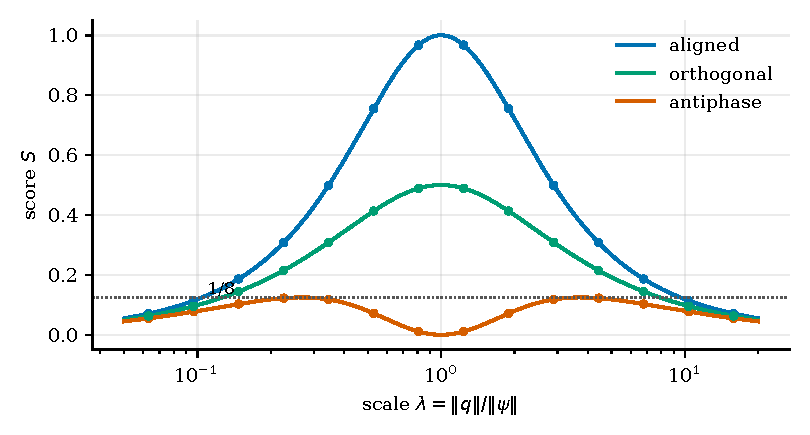
\includegraphics[width=0.85\textwidth]{figs/score_scale}
\caption{Resonance score as a function of the query scale $\lambda$ for an aligned, orthogonal and antiphase query. Curves are the closed form \eqref{eq:Aclosed}; points are the score computed from its definition on random vectors in $\C^8$. The dotted line marks the maximum $1/8$ of the antiphase curve. Computed by the script \texttt{figs.py} with seed 8; an illustration of the stated analytic result and not an evaluation of the architecture.}\label{fig:score}
\end{figure}

\chapter{Phase Transformations and Semantic Operators}\label{ch:operators}

The wave-based proposal names four semantic operators and applies them to base terms. Negation, written NEG, is described as aligning a pattern with antiphased opposites. A controlled phase shift, SHIFT+, is described as producing stable offset clusters. Two amplitude operators, INT\_UP and INT\_DOWN, are described as producing amplitude-driven zones \cite{listopad2025}. The text of the source does not give formulas, phase offsets, or scaling rules for any of them, so the operators cannot be reproduced from the paper alone. The monograph therefore adopts candidate definitions, consistent with the one-line descriptions, and states exactly what each implies for the score. The definitions are a modeling choice made here and are not claimed to be the source's.

\begin{definition}[Candidate operators]\label{def:cand-ops}
For a pattern $\psi\in\Hil$, a phase offset $\delta\in(0,\pi)$, and a scale $\gamma>1$, define $\mathrm{NEG}(\psi)=e^{\iu\pi}\psi=-\psi$, $\mathrm{SHIFT}^+_\delta(\psi)=e^{\iu\delta}\psi$, $\mathrm{INT\_UP}_\gamma(\psi)=\gamma\psi$, and $\mathrm{INT\_DOWN}_\gamma(\psi)=\gamma^{-1}\psi$.
\end{definition}

All four are multiplication by a nonzero complex scalar $\lambda=\gamma e^{\iu\delta}$, and the family of such multiplications is the multiplicative group $\C^\times$ acting on $\Hil$ by scalars. The composition law $U_gU_h=U_{gh}$ required of a group action holds, and the maps are invertible isometries up to scale. The closed form of Theorem~\ref{thm:closed} then gives the score between a pattern and its image in one line.

\begin{proposition}[Score of an operator image]\label{prop:opimage}
For $\psi\ne0$ and $\lambda=\gamma e^{\iu\delta}$, $S(\psi,\lambda\psi)=\frac\rho2(1+\rho\cos\delta)$ with $\rho=2\gamma/(1+\gamma^2)$. Consequently $S(\psi,\mathrm{NEG}\,\psi)=0$, $S(\psi,\mathrm{SHIFT}^+_\delta\psi)=\frac12(1+\cos\delta)$, and $S(\psi,\mathrm{INT\_UP}_\gamma\psi)=S(\psi,\mathrm{INT\_DOWN}_\gamma\psi)=\frac\rho2(1+\rho)$ with the same $\rho$.
\end{proposition}

\begin{proof}
Here $\norm{\lambda\psi}=\gamma\norm\psi$, so $\rho=2\gamma/(1+\gamma^2)$ and $\Re\ip{\psi}{\lambda\psi}=\norm\psi^2\Re\lambda=\norm\psi^2\gamma\cos\delta$, giving $c=\cos\delta$. Substitute into \eqref{eq:closed}; the values for the four operators follow with $(\gamma,\delta)=(1,\pi),(1,\delta),(\gamma,0)$, and $(\gamma^{-1},0)$, noting $\rho(\gamma)=\rho(\gamma^{-1})$.
\end{proof}

Two consequences are worth stating. First, the score cannot distinguish the amplitude-raising operator from the amplitude-lowering operator with reciprocal factors when each is compared against the unmodified base pattern, since the two images are equally distant in the sense of $S$. Whether the two can be distinguished at all depends on the presence of a reference scale elsewhere in the store, which is a property of the encoder and not of $S$. Second, because every candidate operator is a complex scalar, each acts identically on every coordinate pair of the realified space, as a rotation by $\delta$ combined with a scaling by $\gamma$ in each two-dimensional block. This is a one-parameter-pair family inside the real-linear maps of $\R^{2n}$, and a real-valued model that is allowed a single shared rotation-scaling block can represent every one of these operators exactly.

The semantic status of negation requires a separate argument, because the equation $\mathrm{NEG}(\psi)=-\psi$ is a mathematical convenience and not an analysis of negation. Four distinct things have been called negation in the literature on semantics and retrieval. A phase rotation by $\pi$ is an involution, $\mathrm{NEG}\circ\mathrm{NEG}=\mathrm{id}$, which agrees with the classical law that double negation returns the proposition. It is also a linear isometry, which means it maps antonyms to a set of patterns determined entirely by the geometry of the original ones: whatever is close to $\psi$ is sent to something far from $\psi$ and close to $-\psi$. This conflates contrary and contradictory opposition. The contrary of hot is cold, which is a particular alternative, whereas the contradictory of hot is not-hot, which is the whole complement, including lukewarm and cold and a great many unrelated things. A single vector $-\psi$ can stand for the contrary and cannot stand for the complement, because the complement contains patterns that are mutually orthogonal and no single point is close to all of them under any inner-product score. Negation understood as set complement is therefore not a point-to-point map but a point-to-set map, and the pointwise rotation is at best a representative of one of its members. Alternatively, negation may be modeled as a context-dependent transformation in which the effect on the pattern depends on what is being negated and why, which suggests a learned operator indexed by context; or as a relation between propositions in a separate relational structure, with the vector layer holding only the proposition content. The monograph treats the choice among these as an open modeling question to be settled by the discrimination experiments of Part~IX, and it distinguishes in every case between operators that are invertible isometries, such as phase rotations, and lossy semantic operations, such as projections onto a subspace or collapse of a set of alternatives to a representative, which are idempotent and not injective.

\chapter{ResonanceDB as a Baseline Architecture}\label{ch:resonancedb}

The software implementation accompanying the wave-based proposal is called ResonanceDB. As described in the source, patterns are stored in memory-mapped binary segments as real-valued amplitude-phase pairs and converted to complex form on demand; the similarity kernel is deterministic and retrieval is an exact scan, so there is no index and no approximation, with cost $O(NL)$ for $N$ patterns of length $L$ \cite{listopad2025}. The reported configuration uses pattern lengths $L\in\{512,1024\}$, dataset sizes from $10^4$ to $5\times10^5$ patterns, and top-$k$ retrieval with $k\in\{1,10,100\}$. Execution is on a 12-core CPU at 3.6~GHz with 32~GB of memory under Java 22, cold cache, and a fixed 12-thread executor. Two backends are described, a scalar kernel used for all reported latencies and an experimental vectorized kernel that is excluded from the results. The numerical precision of the stored values is not stated. The source reports that no training is involved, since phases are supplied by the encoder or specified procedurally.

The reported latencies at $L=1024$ and $5\times10^5$ patterns, with a heap near 512~MB, are approximately 135~ms mean and 152~ms at the 95th percentile for top-1, 138~ms and 156~ms for top-10, and 145~ms and 163~ms for top-100. The source's text describes latency as scaling linearly with dataset size, while the latency table is reported at one dataset size only, so the scaling claim is not supported by the numbers presented and is treated here as a hypothesis to be tested.

A dimensional check is useful because it indicates what a faithful reproduction must control. A full scan at the reported configuration touches $5\times10^5\times1024=5.12\times10^8$ pattern coordinates. If each coordinate is stored as an amplitude and a phase in 32-bit floating point, the scan reads $5.12\times10^8\times8=4.1$ gigabytes, and a mean latency of 135~ms then corresponds to an effective read rate of about $30$~GB/s; with 64-bit values the rate doubles. These figures are conditional on the unstated precision and on the whole file being read per query, and they are offered only to show that the result is within the range where memory bandwidth, not arithmetic, is the binding constraint, which suggests that implementation overhead and mathematical retrieval cost are not easily separated in this measurement. A second consideration concerns the arithmetic. Evaluating the interference sum for amplitude-phase storage requires $\cos(\phi_1-\phi_2)$ for each coordinate, which is a transcendental evaluation when phases are continuous and a sign when phases are restricted to $\{0,\pi\}$. The source's mapping from real embeddings assigns phase $0$ to nonnegative coordinates and phase $\pi$ to negative ones. Whether the reported latency was measured on patterns with continuous phases, and whether the scalar kernel avoids the trigonometric evaluation, cannot be determined from the text, and a latency measured on binary-phase data would not transfer to dense-phase data. The reproduction protocol of Chapter~\ref{ch:repro} therefore requires latency to be reported separately for binary-phase and continuous-phase stores.

The baseline algorithm is specified here so that every later variant can be defined as a modification of it. In notation, the exact scan computes the score of the query against every stored pattern and returns the indices of the $k$ largest scores.

\begin{Verbatim}[fontsize=\small,frame=single,framesep=2mm]
function resonance_topk(store, q, k):
    Eq <- sum_x |q[x]|^2
    heap <- empty min-heap of size k
    for i in 1..N:
        psi <- store[i]                      # amplitude-phase pairs -> complex
        E   <- sum_x |psi[x]|^2
        if E + Eq == 0:  s <- 0
        else:
            ip <- sum_x Re( conj(psi[x]) * q[x] )
            s  <- (E + Eq + 2*ip) * sqrt(E*Eq) / (E + Eq)^2
        push (s, i) onto heap, keeping the k largest
    return heap sorted descending
\end{Verbatim}

Two separations are made explicit in every later comparison. Mathematical retrieval cost is the count of arithmetic operations and memory reads that the algorithm requires on an idealized machine, here $\Theta(NL)$ reads and multiply-accumulate operations for the exact scan, and implementation overhead is everything else: input and output, memory mapping, thread scheduling, garbage collection, and conversion between storage and compute formats. Approximate indexing changes the first and can change the second in either direction, and an approximate method must be compared with the exact one at matched recall and not at matched latency alone. The energies $E=\sum_x|\psi[x]|^2$ of stored patterns can be cached at write time, which removes one of the three reductions per pattern from the inner loop, and any reported latency should state whether this was done.

\chapter{The Representational Equivalence Problem}\label{ch:equiv}

The claim that phase-aware retrieval offers an advantage over real-valued vector retrieval admits several readings, and the first task is to decide which of them is available. A categorical claim, that complex vectors can express something that real vectors cannot, is false for the following elementary reason.

\begin{theorem}[Realification]\label{thm:realif}
Define $\iota:\C^n\to\R^{2n}$ by $\iota(z)=(\Re z,\Im z)$. Then $\iota$ is an $\R$-linear bijection with $\ip{\iota z}{\iota w}_{\R}=\Re\ip{z}{w}_{\C}$ for all $z,w$, so $\C^n\cong\R^{2n}$ as real inner-product spaces. Multiplication by $\iu$ corresponds under $\iota$ to the orthogonal matrix $J=\begin{psmallmatrix}0&-I\\ I&0\end{psmallmatrix}$, which satisfies $J^2=-I$. A real-linear map $A$ of $\R^{2n}$ is of the form $\iota\circ B\circ\iota^{-1}$ for a complex-linear map $B$ of $\C^n$ if and only if $AJ=JA$.
\end{theorem}

\begin{proof}
Linearity and bijectivity are immediate. For $z=x+\iu y$ and $w=u+\iu v$, $\overline z\,w=(xu+yv)+\iu(xv-yu)$ in each coordinate, so $\Re\ip zw=\sum_k(x_ku_k+y_kv_k)=\ip{\iota z}{\iota w}$. Multiplication by $\iu$ sends $x+\iu y$ to $-y+\iu x$, hence $(x,y)\mapsto(-y,x)=J(x,y)$, and $J^2(x,y)=(-x,-y)$. If $B$ is complex-linear then $B(\iu z)=\iu B(z)$, which reads $AJ=JA$ for $A=\iota B\iota^{-1}$. Conversely, an $\R$-linear $A$ commuting with $J$ commutes with multiplication by $\iu$ and is therefore $\C$-linear.
\end{proof}

\begin{corollary}[Dimension count for the inductive bias]\label{cor:dimcount}
The space of complex-linear maps of $\C^n$ has real dimension $2n^2$, while the space of real-linear maps of $\R^{2n}$ has real dimension $4n^2$. A complex-valued linear layer is therefore a real layer with the constraint $AJ=JA$, which halves the number of free parameters.
\end{corollary}

The relationship between the score and the realification is immediate from Corollary~\ref{cor:bounds}: since $\rho$ and $c$ are functions of norms and of the real inner product, $S(z,w)=S_{\R}(\iota z,\iota w)$ where $S_{\R}(x,y)=\frac\rho2(1+\rho\,\ip xy/(\norm x\norm y))$ is the same formula on $\R^{2n}$. Retrieval over a complex store by $S$ is retrieval over the realified store by $S_{\R}$, with identical rankings.

The comparison made in the source between resonance retrieval and cosine retrieval must therefore be read as a comparison between feature maps, norm treatment, and operators, not as one between number systems. Four candidate sources of advantage can be distinguished, and each has a different experimental signature. The first is the energy-balance factor $\rho$, which is an amplitude-sensitivity that cosine discards and which could be added to a real-valued score without changing the representation. The second is the feature map. The source's mapping from real embeddings $v$ sets $A(x)=|v(x)|$ and $\phi(x)=0$ or $\pi$ according to the sign of $v(x)$, so the complex pattern equals $v(x)$ exactly, a real vector regarded as an element of $\C^n$.
\begin{proposition}[Sign-phase patterns are real vectors]\label{prop:signphase}
If $\psi(x)=|v(x)|e^{\iu\phi(x)}$ with $\phi(x)=0$ for $v(x)\ge0$ and $\phi(x)=\pi$ otherwise, then $\psi(x)=v(x)$ for every $x$. For two such patterns $\psi_u,\psi_v$ generated from real vectors $u,v$, the phase-aware cosine equals the ordinary cosine of $u$ and $v$, and $S(\psi_u,\psi_v)=\frac\rho2(1+\rho\cos(u,v))$.
\end{proposition}
\begin{proof}
For $v(x)\ge0$, $|v(x)|e^{0}=v(x)$; for $v(x)<0$, $|v(x)|e^{\iu\pi}=-|v(x)|=v(x)$. The inner product of two real-valued complex vectors is their real inner product, so $c=\cos(u,v)$.
\end{proof}
On data generated this way, the only difference between $S$ and cosine is the balance factor $\rho$, and for unit-norm embeddings there is no difference at all in ranking. Any measured advantage of resonance over cosine on such data must come either from $\rho$ acting on unequal norms or from the operators, which are the transformations that introduce phases other than $0$ and $\pi$. The third source is the family of operators, which as shown in Chapter~\ref{ch:operators} are complex scalars and so are a structured, low-dimensional subfamily of real-linear maps. A cosine baseline applied to the original real vectors cannot represent a phase offset that the real vectors do not contain, but a baseline applied to the realified vectors can, so a comparison that feeds the baseline only the original embeddings of the base terms and the complex model the operator-transformed patterns is a comparison of information supplied, not of retrieval rules. The fourth source is numerical organization and learning dynamics: the shared structure of complex arithmetic can improve optimization or conditioning when parameters are learned, which is the argument advanced in the literature on complex-valued neural networks \cite{trabelsi2018}, and which cannot arise for a retrieval rule without training.

\begin{theorem}[Matched-baseline principle]\label{thm:matched}
Let $\mathcal D$ be a dataset of complex patterns and queries and let any retrieval task be defined by the set of rankings produced by $S$. Then the realified dataset $\iota(\mathcal D)$ with the score $S_{\R}$ produces identical rankings. Consequently, a statement that resonance retrieval outperforms a real-valued method on $\mathcal D$ is equivalent to a statement that $S_{\R}$ on $\R^{2n}$ outperforms that method on $\iota(\mathcal D)$, and no property of complex numbers is involved beyond the construction of $\mathcal D$.
\end{theorem}

The protocol consequence is a requirement of matched capacity. A complex pattern of length $L$ carries $2L$ real degrees of freedom, so the real-valued baselines in Part~IX are of dimension $2L$ and are given the same encoder outputs, together with versions given only the original embeddings, so that the contribution of the operator-generated phases can be separated from the contribution of the retrieval rule. This chapter is the place where the monograph forecloses the claim of intrinsic mathematical superiority of complex embeddings as a premise. What remains possible is that the inductive bias of a structured operator family, the numerical behavior under learning, or the interpretability of phase as a relational variable provides practical advantages, and those are empirical hypotheses to be tested against matched baselines.
